\documentclass{IEEEtran}

\usepackage{amsmath}
\usepackage{amssymb}
\usepackage{amsfonts}

\ifCLASSINFOpdf
   \usepackage[pdftex]{graphicx}
\else
   \usepackage[dvips]{graphicx}
\fi

\ifCLASSOPTIONcompsoc
  \usepackage[caption=false, font=normalsize, labelfont=sf, textfont=sf]{subfig}
\else
  \usepackage[caption=false, font=footnotesize]{subfig}
\fi

\usepackage{textcomp}
\usepackage{nicefrac}
\usepackage{siunitx}
\usepackage{fancyref}

\usepackage[style=ieee, doi=false, isbn=false, url=false, maxbibnames=1, minbibnames=1, maxcitenames=1, mincitenames=1, backend=biber, defernumbers=false]{biblatex}
\addbibresource{./references.bib}

\usepackage[activate={true, nocompatibility}, final, tracking=true, kerning=true, spacing=true, factor=1100, stretch=10, shrink=10]{microtype}
\linespread{0.95}

\usepackage{glossaries}
\newacronym{AE}{AE}{Auto-Encoder}
\newacronym{AC}{AC}{Attenuation Correction}
\newacronym{ALS}{ALS}{Amyotrophic Lateral Sclerosis}
\newacronym{GPU}{GPU}{Graphics Processing Unit}
\newacronym{FDG}{FDG}{FluoroDeoxyGlucose}
\newacronym{AIF}{AIF}{Arterial Input Function}
\newacronym{AUC}{AUC}{Area Under the Curve}
\newacronym{cLBP}{cLBP}{chronic Low Back Pain}
\newacronym{CV}{CV}{Cofficient of Variation}
\newacronym{MSE}{MSE}{Mean Squared Error}
\newacronym{MR}{MR}{Magnetic Resonance}
\newacronym{PBR28}{[$^{11}$C]-PBR$28$}{[$^{11}$C]-Peripheral Benzodiazepine Receptor}
\newacronym{MNI}{MNI}{Montreal Neurological Institute}
\newacronym{FWHM}{FWHM}{Full Width Half Maximum}
\newacronym{HC}{HC}{Healthy Control}
\newacronym{HAB}{HAB}{High Affinity Binder}
\newacronym{MAB}{MAB}{Mixed Affinity Binder}
\newacronym{PT}{PT}{Patient}
\newacronym{HPLC}{HPLC}{High Performance Liquid Chromatography}
\newacronym{IDIF}{IDIF}{Image Derived Input Function}
\newacronym{LL}{LL}{Log-Likelihood}
\newacronym{LSTM}{LSTM}{Long Short Term Memory}
\newacronym{KOA}{KOA}{Knee Osteo-Arthritis}
\newacronym{MAE}{MAE}{Mean Absolute Error}
\newacronym{ML}{ML}{Machine Learning}
\newacronym{NN}{NN}{Neural Network}
\newacronym{SUV}{SUV}{Standardised Uptake Value}
\newacronym{TAC}{TAC}{Time Activity Curve}
\newacronym{OSEM}{OSEM}{Ordered Subset Expectation Maximisation}
\newacronym{PET}{PET}{Positron Emission Tomography}
\newacronym{ROI}{ROI}{Region Of Interest}
\newacronym{RMSE}{RMSE}{Root Mean Squared Error}
\newacronym{TSPO}{TSPO}{Translocator Protein 18 kDa}
\newacronym{TCM}{TCM}{Tissue Compartment Model}
\newacronym{SNR}{SNR}{Signal to Noise Ratio}
\newacronym{mCi}{mCi}{Millicurie}
\newacronym{VT}{V$_{\mathrm{T}}$}{Volume of Distribution}
\newacronym{IF}{IF}{Input Function}
\newacronym{NLP}{NLP}{Natural Language Processing}

% \markboth{IEEE TRANSACTIONS ON NUCLEAR SCIENCE, VOL. XX, NO. XX, XXXX 2020}
% {Author \MakeLowercase{\textit{et al.}}: Preparation of Papers for Review by the \textsc{IEEE Transactions on Nuclear  Science} \newline (May 2020)}

\usepackage{lipsum}

\begin{document}
\title{
    \vspace{-0.75cm}
    
    A Bayesian Neural Network-Based Method For The Extraction Of A Metabolite Corrected Arterial Input Function From Dynamic [$^{11}$C]PBR28 PET 
}

\author{
    \vspace{-0.25cm}
    
    Alexander C. Whitehead$^{*}$,
    Ludovica Brusaferri$^{*}$,
    Lucia Maccioni,
    Matteo Ferrante,
    Marianna Inglese,
    Zeynab Alshelh,
    Mattia Veronese,
    Nicola Toschi,
    Jodi Gilman,
    Kris Thielemans, and
    Marco L. Loggia

    \vspace{-0.75cm}
    
    \thanks{This work was funded by the NIH grants R01-NS094306-01A1, R01-NS095937-01A1 and R01-DA047088-01, GE Healthcare, the NIHR UCLH Biomedical Research Centre and the UCL EPSRC Centre for Doctoral Training in Intelligent, Integrated Imaging in Healthcare (i4health) grant (EP/L016478/1) and by the Open Source Imaging Consortium (OSIC).}
    \thanks{Alexander~C.~Whitehead was with the Institute of Nuclear Medicine, University College London, London, UK and the Centre for Medical Image Computing, University College London, London, UK. He is now with the Department of Computer Science, University College London, London, UK.} 
    \thanks{Ludovica~Brusaferri, is with Athinoula A. Martinos Center for Biomedical Imaging, Harvard Medical School, Boston, MA, US.}
}

\pagestyle{plain}
\pagenumbering{gobble}

\maketitle

\begin{abstract}
    Arterial blood sampling is the gold standard for input function measurements in PET imaging, especially for such tracers as [$^{11}$C]PBR28 that produce radio-metabolites. As arterial sampling is an invasive procedure, its application is limited in routine clinical practice. Here we propose a deep learning-based method to directly estimate the input function from dynamic PET images (NN-AEIF), as well as to metabolite-correct the IDIF (NN-IDIF) and the un-corrected  plasma curve (NN-AIF). All the NN-based methods output a measure for prediction uncertainty. The three methods (together with IDIF) were compared to the metabolite-corrected AIF in terms of V{$_\mathrm{T}$}, while the uncertainty of each NN-based method was assessed in terms of CV. Overall, both NN-AEIF and NN-AIF were able to accurately predict V{$_\mathrm{T}$}s, outperforming the other methods, with NN-AEIF showing the lowest  CV.
\end{abstract}

% \begin{IEEEkeywords}
% Enter key words or phrases in alphabetical
% \end{IEEEkeywords}

\vspace{-0.6cm}

\section{Introduction} \label{sec:introduction}\vspace{-0.3cm}\vspace{0.2cm}
    \IEEEPARstart{T}{he} \gls{VT} estimated with an \gls{AIF} is utilised for  quantification of many \gls{PET} tracers including \gls{PBR28}. This, however, requires the concurrent measurement of the concentrations of unchanged radioligand in arterial plasma. Although insertion of an arterial catheter rarely results in clinically relevant adverse events, it is an invasive and laborious procedure. 
    \gls{IDIF} represents a promising alternative to arterial sampling~\cite{Zanotti-Fregonara2011}. However, its applicability in clinical research is hampered by several reasons including the inaccuracy in the estimation of both shape and amplitude of the \gls{IF}; moreover \gls{IDIF} does not allow for radio-metabolites quantification~\cite{Sari2018Non-invasive11C-SB201745}. The application of \gls{ML} is expected to improve the accuracy of predicting the \gls{AIF} from \gls{PET} images~\cite{Kuttner2020, Ferrante2022PhysicallyImaging}. While those methods have shown promising results, the vast majority of those approaches have been developed for \gls{PET} tracers that do not have radio-metabolites. Moreover, even if the developed model shows sufficient prediction accuracy for unseen data, it remains challenging to trust  in clinical settings. Here, we propose a bayesian \gls{NN}-based method for predicting a metabolite corrected \gls{AIF}, while allowing for the estimation of uncertainty of the model's output.%Specifically for the \gls{AE}, although also present in the other networks, we try to enforce the low dimensional representation of the input data as disentangled and continuous. Furthermore, the network does not predict a single signal for each input; rather, it predicts a probability density function of potential signals, which allows for the estimation of uncertainty of the model's output.
    
    % it can be applied retrospectively, it isn't prone to user error, it can be used to save scans where the blood has failed, sites require blood sampling facilities and staff

%\vspace{-0.5cm}

\section{Methods} \label{sec:methods} 
\vspace{-0.15cm}
    \subsection{Data acquisition and processing}\label{sec:dataproc}
        Dynamic \gls{PBR28} \gls{PET}/\gls{MR} images from $52$ individuals (Age: $55 \pm 16$ years; Sex: $27$ Male, $25$ Female; Genotype: $32$ \glspl{HAB}, $20$ \glspl{MAB}; Clinical population: $12$ Healthy Controls, $40$ Chronic Pain patients; Injected Dose: $14.16 \pm 1.3$ \glspl{mCi}) were acquired on a Siemens Biograph mMR whole-body tomograph for a time-period of $0$-$90$ minutes post-injection. Data were pooled for multiple protocols (approved by the Partners Healthcare/Mass General Brigham Institutional Review Board) and reconstructed as in \cite{Brusaferri2022ThePandemic}. All subjects received a radial artery catheter at the time of the scan. Uncorrected plasma curves from the blood samples were interpolated and metabolite-corrected to obtain the \gls{AIF}. %Uncorrected plasma curves were obtained from raw blood samples using linear fitting. In $16$ subjects, arterial blood processing was performed using a HyperSep C$18$ solid extraction cartridge to separation of radio-metabolites; in $36$ subjects, \gls{HPLC} for separation of radio-metabolites from parent radiotracer was used instead. Hill-fitted parent fractions were applied to the raw data and a radio-metabolite-corrected \gls{AIF} was obtained for each subject. Previous cross-validation confirmed reliability of both pipelines allowing for the combination of both data-sets to increase statistical power of the study~\cite{Brusaferri2022ThePandemic}. 
        
        For validation purposes, \gls{IDIF} was also calculated by segmenting the arterial carotid siphons via intensity thresholding of early  dynamic \gls{PET} frames. Data were split following ten-fold cross validation. The split was specifically designated to maximise the within-variance while minimising the between-variance in training and testing sets.

    \vspace{-0.5cm}
    
    \subsection{Neural Network Design}\label{sec:NNDesign}
        The method comprises of three independent \glspl{NN}: \gls{NN}$_1$ seeks to reduce the dimentionality of the input data (due to computational requirements) and extract the most relevant features. \gls{NN}$_2$ aims to extract a non-metabolite corrected signal from the low-dimensional representation output by the first network. \gls{NN}$_3$ metabolite corrects the non-metabolite corrected signal. Details follow in the next sections.
        %All models use a novel activation function, defined as $PSoftplus = \log\big(\mathrm{e}^{x} + \alpha^2 \big)$, where $x$ is the output from the previous layer and $\alpha$ is a learnt parameter which is initialised as $\alpha = 0$.  This activation function was designed as a fully differentiable drop-in replacement for \textit{PReLU} \cite{Ciuparu2020Soft++Architectures}. The initial value of $\alpha$ is selected such that the activation is initially linear (thus making the model easier to train at early iterations) and becomes non-linear as training progresses.
        % https://www.sciencedirect.com/science/article/pii/S0925231219317163

        %In order to try to enforce disentanglement and continuity of this layer, a regularisation term to enforce the orthogonality of its output was used. To promote stability of the optimisation, a regularisation term which compares the area under the curve of the prediction and true signals was used in each \gls{NN}. Common to all \glspl{NN}, each model was optimised using AdaBelief~\cite{Zhuang2020AdaBeliefGradients} with the warm-up proportion equivalent to one-tenth of the total number of epochs, after which it does not decrease. Weight decay was used to regularise against large weights. %Each model was trained initially using \gls{RMSE}, where the mean output of the model is penalised against the expected value and the standard deviation output of the model is encouraged to be close to $1$. Subsequently, a second training regime was used where the negative \gls{LL} function is used to fine-tune the parameters. Gradient accumulation was used to allow for only one data-point to be loaded onto the \gls{GPU} at any one time and for any arbitrary batch-size to be used. The batch size starts at two and increases to the size of total number of data points, where the batch size doubles as the current epoch number quadruples.

        \subsubsection{\gls{NN}$_1$ \gls{AE}} \label{sec:NN1}
            This network consists of three blocks, the downsampling block, the latent layer, and the upsampling block. The downsampling block comprises three convolutions, all with kernel size equal to three, and where the final convolution has a stride of two. The latent block is flanked on either side by two convolutions, with a variational latent layer in the middle. The upsampling block consists of a transposed convolution and two standard convolutions, all with kernel size equal to three, and where the transposed convolution has a stride of two. The mean and standard deviation of the latent layer and final layer are output from the model and passed onto \gls{NN}$_2$.
            Each time frame was treated as an independent training example.

            %The target images were smoothed using a Gaussian filter with a \gls{FWHM} equal to three times the voxel size in each dimension. All images were padded such that the size of each dimension was equal to the next larger power of two. Both input and target images were standardised separately, based on parameters obtained from the training set.

        \subsubsection{\gls{NN}$_2$ Signal Extractor} \label{sec:NN2}
            This network consists of three blocks, the downsampling block, the latent layer and the fully connected block. The downsampling block follows the same structure as in \gls{NN}$_1$. The fully connected block consists solely of one fully connected layer. All time frames were used simultaneously, where the same convolutions are applied independently on the image of each time frame before global average pooling and flattening. Both input and target data were standardised separately, based on parameters obtained from the training set. 
        \subsubsection{\gls{NN}$_3$ Metabolite Correction and Reshaping} \label{sec:NN3}
            This network consists solely of fully connected layers. If the network is to metabolite-correct a signal (e.g. from \gls{AIF} or \gls{IDIF}), it takes that signal as input together with the clinical features (age, sex, genotype, injected dose, clinical population).  If the network is instead to correct a signal obtained with \gls{NN}$_2$, both the mean and the standard deviation of the uncorrected signal are input to \gls{NN}$_3$, in addition to the latent layer from \gls{NN}$_2$. %The input data was preprocessed in the same way as for \gls{NN}$_2$.

            %Both input and target data are standardised separately, based on parameters obtained from the training set. Only the mean was standardised. Each element of the clinical features was either standardised or encoded using one hot encoding depending on the nature of the feature. Because the autoencoder outputs both a mean and a standard deviation values were sampled at the input of the network using the same \textit{reparametrisation-trick} as for a variational autoencoder.

    \vspace{-0.44cm}
    
    \subsection{Evaluation}\label{sec:evaluation}
    \vspace{-0.1cm}
        %The mean and standard deviation were sampled $32$ times (to satisfy the central limit theorem) from the model and the output was sampled $32$ times from the mean of these to acquire multiple realisations of the estimated signal. 
        %Then, candidate signals from~\Fref{sec:candidates} were compared in terms of \glspl{VT}, calculated via Logan graphical method, for each realisation of the output (\Fref{sec:metrics}), in $69$   \glspl{ROI}.

        \subsubsection{Metrics} \label{sec:metrics}
         The model was sampled $32$ times resulting in multiple realisations of the estimated signal. Then, $V_{\mathrm{T}} \in \mathbb{R}^{r \times s \times b}$ were computed via Logan graphical method, where $r$ is the number of \glspl{ROI} ($r = 69$), $s$ is the number of subjects ($s = 5$) and $b$ is the number of model samples ($b = 32$). For both AIF and IDIF, $b=1$. For the \gls{NN}-based methods, \glspl{VT} were computed for each model realisation and then used to calculate the mean \gls{VT} and its standard deviation.
        Moreover, the \gls{CV} was defined as $\mathrm{CV} = \mathrm{std} ( Pred \; V_{\mathrm{T}} ) / True \; V_{\mathrm{T}}$ with $\mathrm{CV} \in \mathbb{R}^{r \times s }$.

        \subsubsection{Statistical Analyses} \label{sec:stats}
        For each candidate signal, correlation analyses were performed to compare the \glspl{VT} (computed for all the \glspl{ROI} and for all the subjects in the test-set) to the ones obtained with the ground truth signal (\textbf{TRUE-AIF}, see~\Fref{sec:dataproc}). To measure the accuracy of the prediction, the angle between the regression- and the identity-line was also computed, defined as $\theta = 45 - \arctan(m)*180/\pi$, with $m$ being the slope of the regression-line.
        Furthermore, \glspl{CV} were averaged across \glspl{ROI} for each subject of the test-set and compared via a paired t-test for each of the three \gls{NN}-based methods.
       
        \subsubsection{Candidate signals} \label{sec:candidates}
            \begin{itemize}
                \item \textbf{\gls{NN}-\gls{AIF}} - metabolite-corrected \gls{AIF} obtained from (uncorrected) arterial plasma input to \gls{NN}$_3$~\Fref{sec:NN3}.
                \item \textbf{\gls{NN}-\gls{AE}\gls{IF}} - metabolite-corrected \gls{IF} obtained from dynamic \gls{PET} images input to \gls{NN}$_{1,2,3}$~\Fref{sec:NN1} - \Fref{sec:NN3}.
                \item \textbf{\gls{NN}-\gls{IDIF}} - metabolite-corrected \gls{IF} obtained from \gls{IDIF} input to \gls{NN}$_3$~\Fref{sec:NN3}.
                \item  \textbf{\gls{IDIF}} - generated as in~\Fref{sec:dataproc}.
            \end{itemize}

\vspace{-0.5cm}

\section{Results} \label{sec:results}
    \begin{figure}
        \vspace{-0.5cm}
        
        \centering
        
        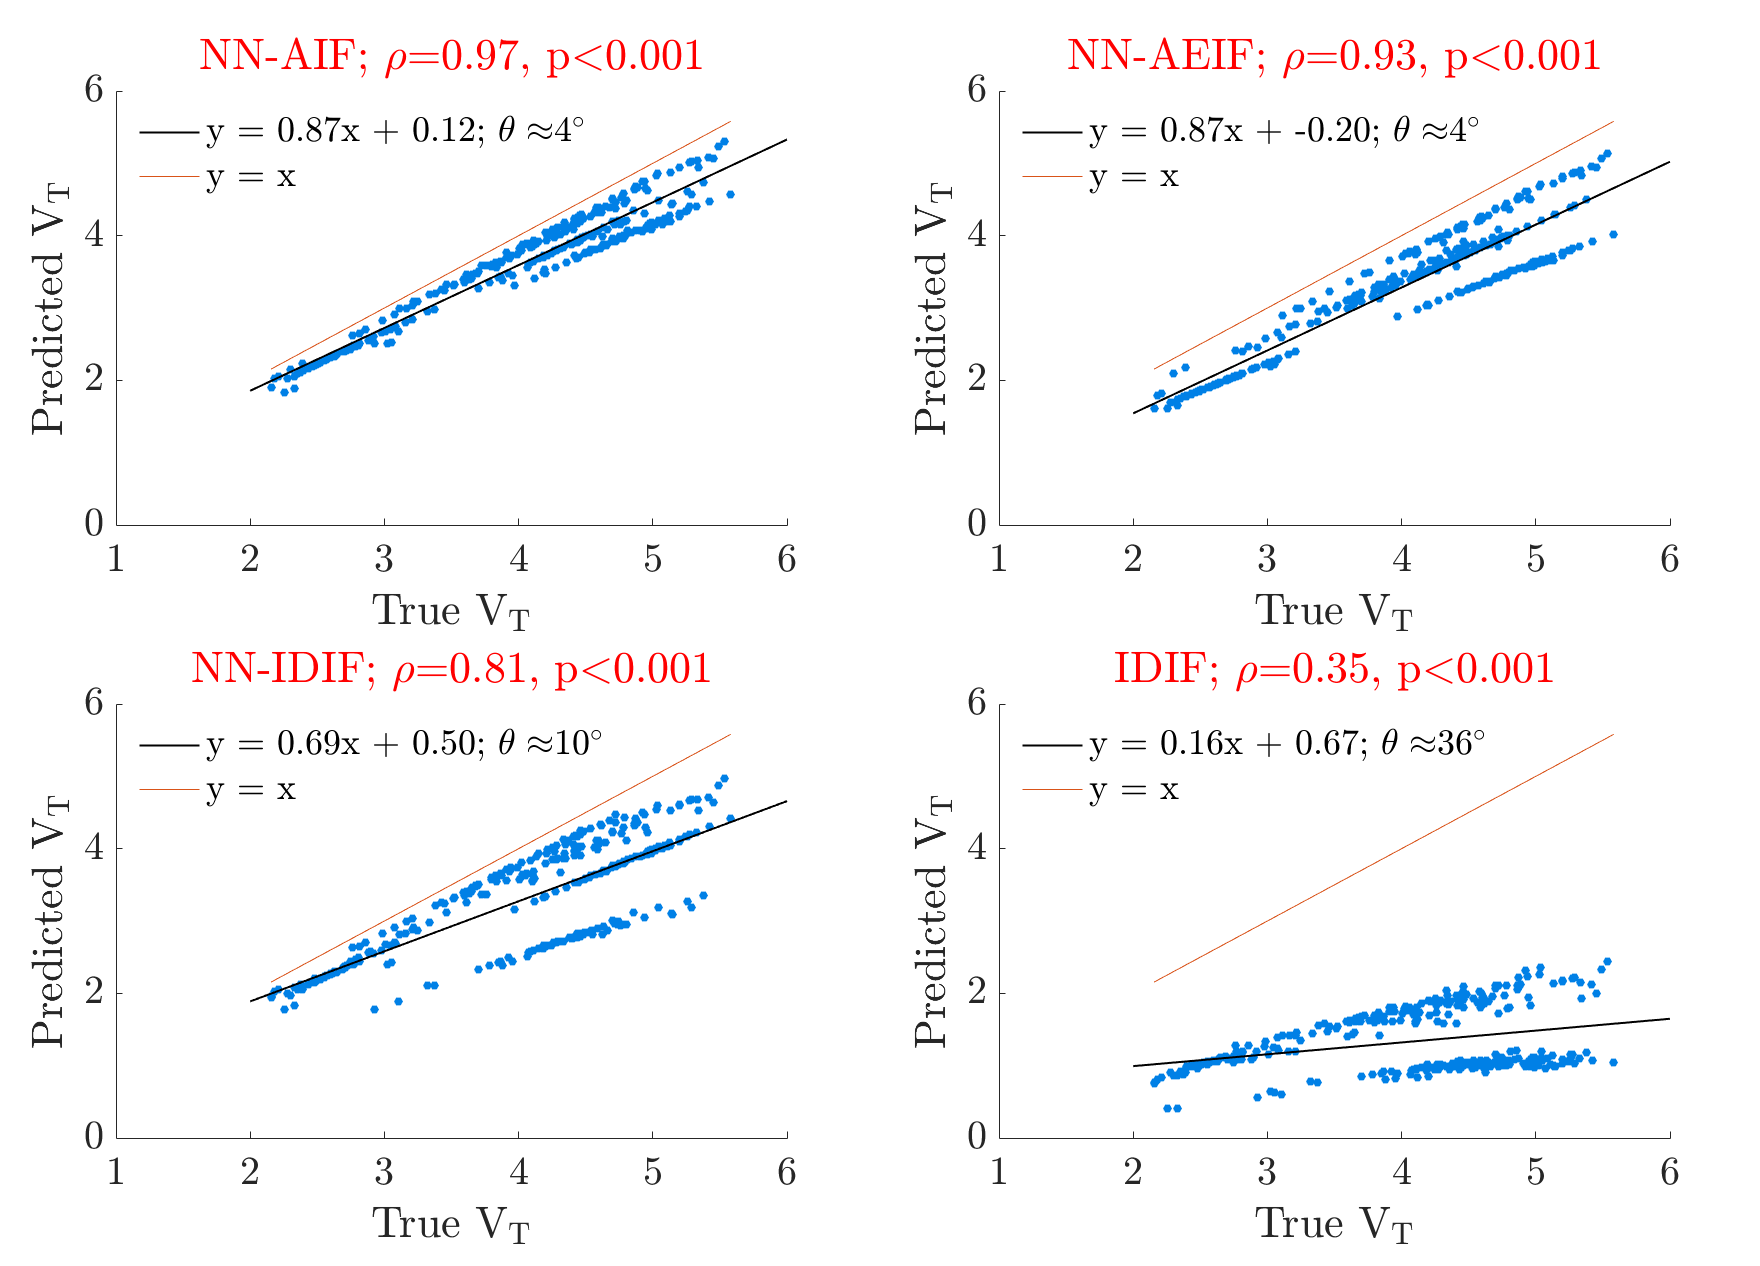
\includegraphics[width=1.0\linewidth]{Figures/correlation.png}
        
        \vspace{-0.25cm}
        
        \captionsetup{singlelinecheck=false, justification=centering}
        \caption{
            \scriptsize
            Predicted $V_{\mathrm{T}} \in \mathbb{R}^{r \times s}$ in the test-set subjects, with $r = 69$ and $s=5$ estimated with the four candidate signals, correlated to the True \gls{VT} (obtained with TRUE-\gls{AIF}). Please note that for the \gls{NN}-based methods, the displayed \glspl{VT} was averaged over all multiple realisations.
        }
        
        \label{fig:correlation}
        
       % \vspace{-0.5cm}
   \end{figure}

    \begin{figure}
        %\vspace{-0.5cm}
        
        \centering
        
        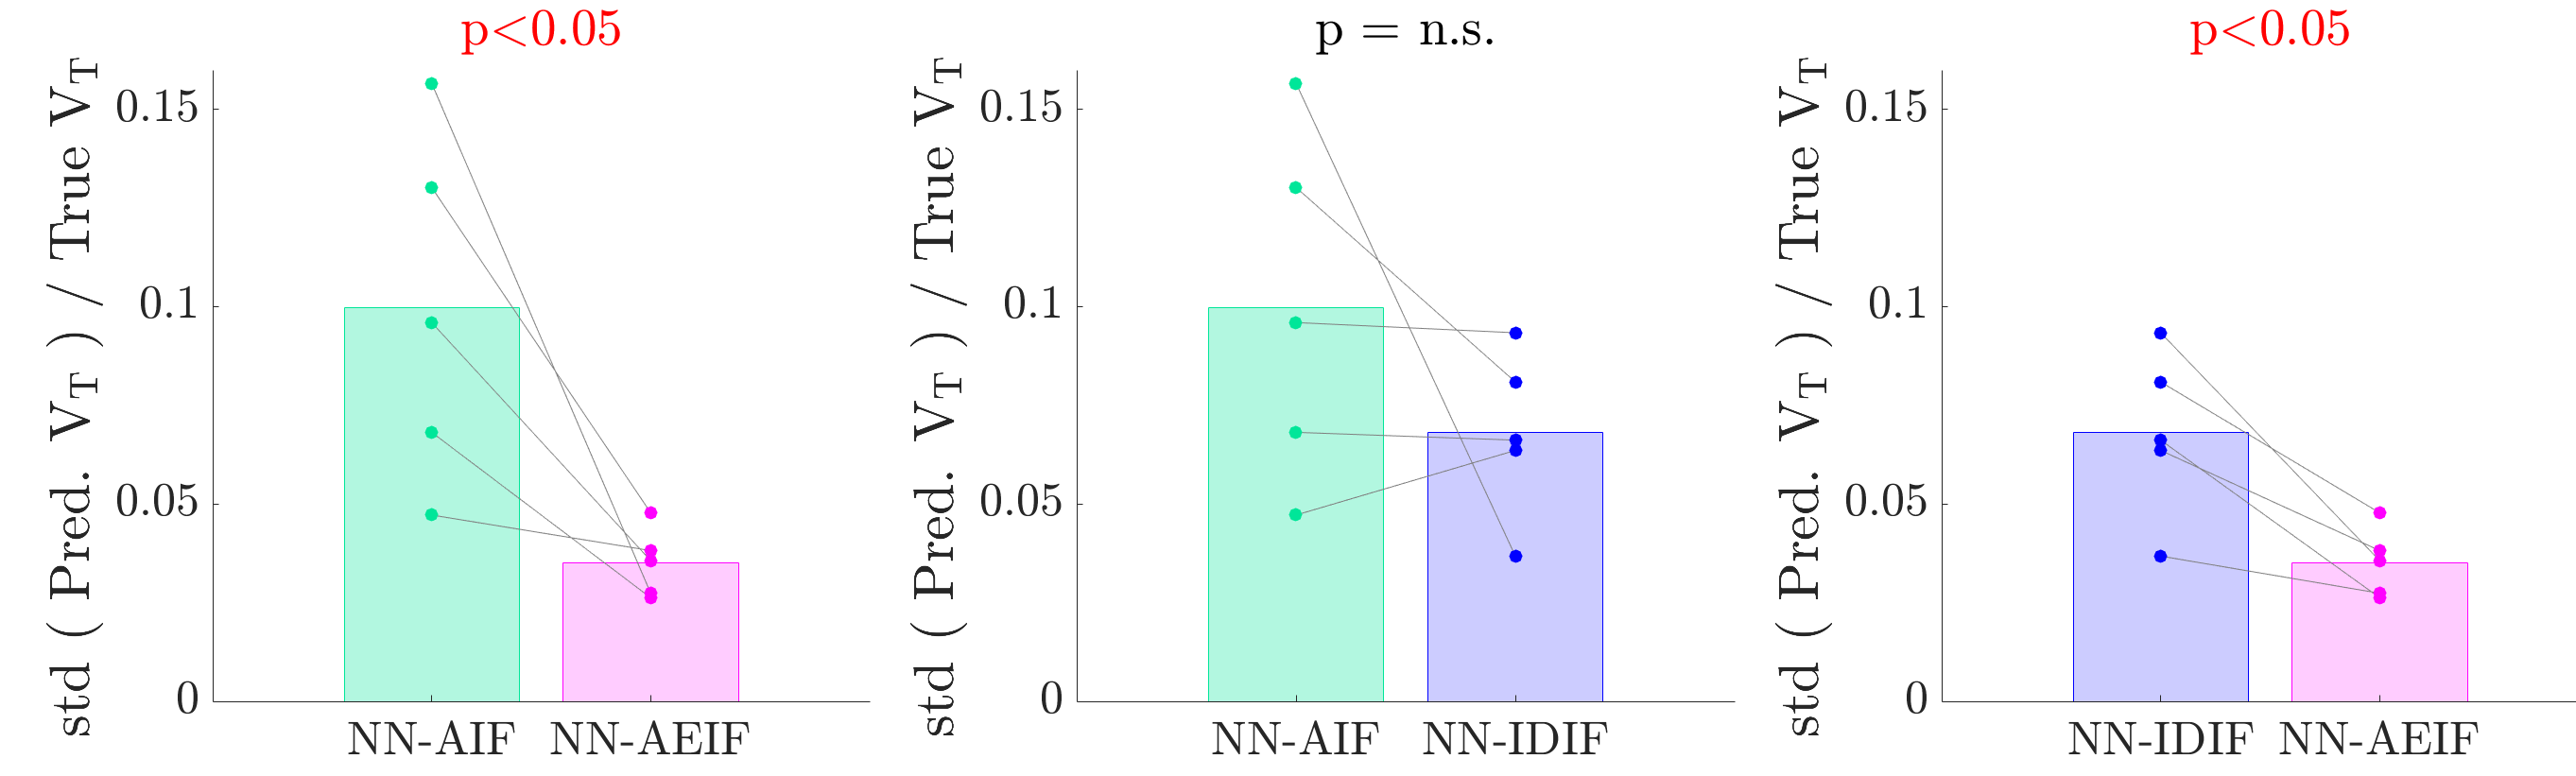
\includegraphics[width=1.0\linewidth]{Figures/CVar.png}
        
        \vspace{-0.25cm}
        
        \captionsetup{singlelinecheck=false, justification=centering}
        \caption{
            \scriptsize
            Paired t-test comparing \glspl{CV} across the three \gls{NN}-methods for the test-set subjects. 
        }
        
        \label{fig:CVar}
        
        \vspace{-0.5cm}
   \end{figure}
   
   \Fref{fig:correlation} reports the correlation analyses between the predicted \gls{VT} values (obtained by the four candidate methods) and the true \gls{VT}. For all methods, predicted \gls{VT} values positively correlate with true \gls{VT}, with \gls{NN}-\gls{AIF} and \gls{IDIF} showing the highest and the lowest Pearson correlation coefficient ($\rho$), as well as the smallest and largest angular distance to the identity line respectively: $\rho = 0.97 \; \& \;  \theta \approx 4^{\circ}$ vs $\rho = 0.35 \; \&  \; \theta \approx 36^{\circ}$. Overall, \gls{NN}-\gls{AE}\gls{IF} slightly outperforms \gls{NN}-\gls{IDIF} in terms of Pearson correlation coefficient and angular distance: $\rho = 0.93 \; \& \; \theta  \approx 4^{\circ}$ vs $\rho = 0.81 \; \&  \; \theta \approx 10^{\circ}$.

    With regard to the variance analysis, \gls{NN}-\gls{AE}\gls{IF} outperforms both \gls{NN}-\gls{AIF} and \gls{NN}-\gls{IDIF}, showing the lowest \gls{CV}, while \gls{NN}-\gls{AIF} and \gls{NN}-\gls{IDIF} do not differ in terms of \gls{CV} values (\Fref{fig:CVar}).

\vspace{-0.5cm}

\section{Discussion And Conclusion} \label{sec:discussion}
    This work proposes a Bayesian \gls{NN}-based approach to estimate the \gls{AIF} from dynamic \gls{PET} images and clinical variables (i.e. age, sex, \gls{TSPO} genotype, injected dose, clinical population). This approach has similarities with previous methods developed for \gls{PET} tracers that do not produce radio-metabolites, such as [$^{18}$F]\gls{FDG}. Here, additional efforts were devoted to deal with \gls{PBR28} radio-metabolite correction, as population-based approaches cannot account for between-subjects variability~\cite{Mertens2021MinimallyFunction}. Moreover, the proposed method seeks to estimate not only a signal but also its uncertainty, which can provide a measure of confidence in the generated signal for unseen data, as well as be used in further computations. Additionally, not only this method extracts a signal and metabolite-corrects it, but because the method is split in multiple parts, each part can be used independently; for instance, here where metabolite correction was applied to a signal generated by a more traditional method (\gls{IDIF}).  The four candidate signals, seen in~\Fref{sec:candidates}, were compared to the gold standard TRUE-\gls{AIF}, obtained from arterial blood sampling and metabolite correction. Overall, \gls{NN}-\gls{AE}\gls{IF} showed comparable performance in terms of correlation and bias to \gls{NN}-\gls{AIF}, with the lowest variance of the estimated \gls{VT}, as measured by the \gls{CV}. This can potentially be explained by the amount of input data being larger and thus the model itself having more parameters.
    
    Interestingly, \gls{NN}-\gls{IDIF} was able to improve on the \gls{IDIF} approach, as demonstrated by a higher correlation coefficient and lower angular distance from the identity line. 
    
    The proposed approach has several limitations, including the small training size which did not allow to assess the accuracy of the prediction within subsets of clinical populations in the test-set (i.e. patients vs healthy controls). 
    
    In the future, the accuracy of the model could be improved through the inclusion of an attention layer either before or after the latent layer of the \gls{AE}, validated through the use of an ablation study. 


\vspace{-0.5cm}

\AtNextBibliography{\scriptsize}
\printbibliography
\end{document}
